\documentclass[14pt, a4paper]{article}  % add twocolumn if you wanna
\usepackage[utf8]{inputenc}
\usepackage[T1]{fontenc}
\usepackage[margin=0.9in, marginpar=0.7in]{geometry} 
\usepackage[font={footnotesize,it}]{caption}
\usepackage{amsmath,amsthm,amssymb,amsfonts, fancyhdr, color, comment, graphicx, environ}
%\usepackage{xcolor}
%\usepackage{mdframed}
\usepackage[shortlabels]{enumitem}
%\usepackage{indentfirst}
%\usepackage{simpler-wick}
\usepackage{booktabs}
%\usepackage{siunitx}
\usepackage{physics}
%\usepackage{polynom}
%\usepackage{verbatim}
%\usepackage{tensor}
\usepackage{todonotes}
%\usepackage{dcolumn}% Align table columns on decimal point
\usepackage{listings}
\usepackage{caption}
\usepackage{subcaption}
\usepackage[backend = biber, style = vancouver]{biblatex}
\bibliography{refs.bib}
% \captionsetup[figure]{skip=-2pt}  % Adjust the skip before and after figure captions
% \captionsetup[table]{skip=-2pt}  % Adjust the skip before and after figure captions
\usepackage{hyperref}
\hypersetup{
    colorlinks=true,
    linkcolor=blue,
    filecolor=magenta,      
    urlcolor=cyan,
    citecolor=cyan,
    }


\title{Higher order asymptotics method to check if toys are needed in low sample statistics in High Energy Physics}
\author{Ruben Guevara, Alexander Lincoln Read}
% \date{February 2024}

\begin{document}
% \twocolumn[  
	% \begin{@twocolumnfalse}
	\maketitle\vspace*{-10mm}
            \begin{abstract}
                Placeholder
		\end{abstract}
		% \end{@twocolumnfalse}
% ]	


\section{Introduction}
Placeholder


\section{Theory}
The main idea behind this is to use the likelihood test statistic, $t_\mu$ to calculate the p-value of a sample in the low sample statistics regime. This works applied the methods showcased by Brazzale et al in the book "Applied Asymptotics: Case Studies in Small-Sample Statistics" \cite{Brazzale_Davison_Reid_2007}. In this book, Brazzale et al, make higher order approximations to the asymptotic of the likelihood root
\begin{equation}\label{eq:likelihood_root}
    r(\theta, \hat{\theta}) = \text{sign}(\hat{\theta}-\theta)\left[2\left\{\ell(\hat{\theta})-\ell(\theta)\right\}\right]^{1/2}
\end{equation}
where $\ell(\theta)$ is the log-likelihood of a distribution at a POI $\theta$ that we wish to do inference on. $\hat\theta$ is the MLE which is found by finding $\theta$ when setting
$$
\frac{\partial \ell(\theta)}{\partial\theta} \overset{!}{=} 0.
$$
As we expect under suitable conditions, and as the sample size $n\rightarrow\infty$, the likelihood root has an asymptotic standard normal $\mathcal{N}(0,1)$. The likelihood root in Eq. (\ref{eq:likelihood_root}) is the root of the likelihood test statistic 
\begin{equation}\label{eq:test_stat}
    t_\theta = r(\theta)^2 = 2\left\{\ell(\hat{\theta})-\ell(\theta)\right\},
\end{equation}
which in particle physics we usually use the notation $t_\mu$ instead.\footnote{Additionally, since we are interested in excess over a  certain hypothesis, we set the values where $\hat\theta\leq\theta$ as a delta function. This replaces $\text{sign}(\hat{\theta}-\theta)$ in Eq. (\ref{eq:likelihood_root}), as Cowan and Cramner showed in ...}. Which, again, under suitable conditions and as the sample size is large, has an asymptotic $\chi^2_1$ distribution.

However, what we are interested in is on the possibility to approximate our test statistics to this under less favorable conditions. The first order asymptotic approximation Brazzale et al make to the likelihood root, is as follows
\begin{equation}\label{eq:first_approx}
    r^*(\theta)=r(\theta)+\frac{1}{r(\theta)}\log\left\{\frac{q(\theta)}{r(\theta)}\right\},
\end{equation}
where this $q(\theta)$, for the context so far, is the \textit{Wald statistic}
\begin{equation}\label{eq:Wald_stat}
    t(\theta)=j(\hat\theta)^{1/2}(\hat\theta - \theta).
\end{equation}
where $j(\theta)$ is the observed information function, defined as
$$
j(\theta) = -\frac{\partial^2 \ell(\theta)}{\partial\theta^2}
$$
(where these may be defined by replacing $j(\hat\theta)$ by $j(\theta),i(\hat\theta)$ or $ i(\theta)$, where $i(\theta)=\mathbb{E}[j(\theta)]$). 

\section{Application}
In particle physics we are performing counting experiments that follow a Poisson distribution. The pmf. of the Poisson is as follows
\begin{equation}\label{eq:poisson_pmf}
    f(y|\theta) = e^{-\theta}\frac{\theta^y}{y!}
\end{equation}
where, for our purposes $y\in\mathbb{N}$ is how many events are in a sample, and $\theta$ is the POI, which is the mean of the distribution. 
The log-likelihood of $n$ iid. samples following the Poisson distribution is
\begin{equation}\label{eq:poisson_ell}
    \ell(\theta) = -n\theta + \sum_i^n y_i\log(\theta) - \log(y_i!),
\end{equation}
giving
$$ 
\frac{\partial \ell(\theta)}{\partial\theta} = -n + \frac{\sum_i^n y_i}{\theta}
$$
giving the MLE
\begin{equation}\label{eq:poisson_MLE}
    \hat{\theta} = \frac{1}{n}\sum_i^n y_i,
\end{equation}
and observed information function
$$
j(\theta) = \frac{1}{\theta^2}\sum_i^n y_i
$$
An interesting quantity we will look at is the p-value for a sample. As we are using the Poisson distribution, we can get the p-value starting from the cdf. The cdf. of a Poisson gives us $\Pr(Y\leq y|\theta)$, we can use the cdf. to calculate the survival function
$$
\Pr(Y>y|\theta) = 1 - \Pr(Y\leq y|\theta),
$$
which is close to the p-value. But as the Poisson is a discrete distribution we can subtract 1 to $y$, giving us
$$
\Pr(Y\geq y|\theta) = \Pr(Y>y-1|\theta),
$$
which is the statistical upper limit, or p-value in the HEP notation. As we will use asymptotics in this study, that means that we can use the likelihood root as an argument for the standard normal cdf., $\Phi(\cdot)$, to get these values. Meaning that using this notation, we will use
\begin{equation}\label{eq:p-val}
    p(\theta) = 1 - \Phi(r^*(\theta, \hat\theta - 1)).
\end{equation}

\subsection{Poisson example as the book}
In the book they explore this method using one sample from the top quark discovery, where $y=27$ and $\theta=\mu+b$ with $b=6.7$. Which when using Eq. (\ref{eq:poisson_MLE}) gives $\hat{\theta}=y$. From this they got 
$$
r(y,\theta) = \text{sign}(y-\theta)[2\{y\log(y/\theta)-(y-\theta)\}]^{1/2},
$$
and \todo{NEED TO UNDERSTAND WHY}
$$
t(y,\theta)=y^{1/2}\log(y/\theta)
$$
With this they plotted the cdf. using the modified likelihood-root using this and the Mid-p \todo{reference, or explanation?} approximation for the background-only hypothesis ($\mu=0$). The result is shown in Figure  \ref{fig:book_cdf}.
\begin{figure}[!ht]
	\centering
        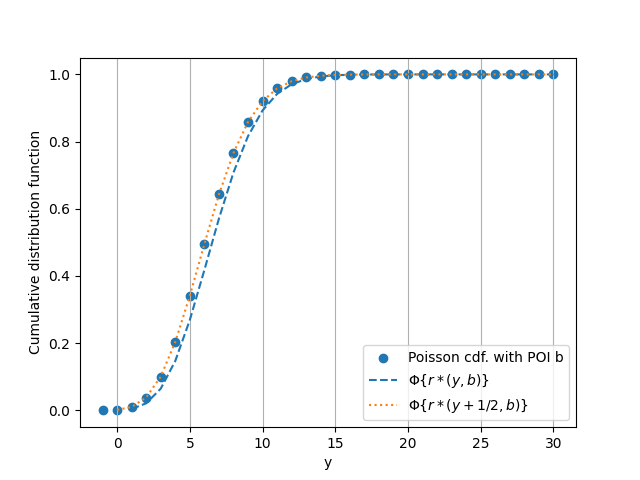
\includegraphics[width=0.7\textwidth]{Book_examples/book_cdf.png}
	\caption{Cumulative distribution function for Poisson distribution with parameter $b=6.7$ (scatter) with approximation $\Phi\{r^*(y,b)\}$ (dashed) and $\Phi\{r^*(y+1/2,b)\}$ (dotted)}\label{fig:book_cdf}
\end{figure} 
Additionally to this, they compare the upper and lower limit of the exact Poisson for the observed events $y=27$ for the background only hypothesis to the approximations. Here they get
\begin{table}[!ht]
    \centering
    \begin{tabular}{l|c}
         Exact upper limit & $29.83\times10^{-10}$ \\
         Exact lower limit & $7.06\times10^{-10}$ \\
         Mid-P $r^*$& $18.45\times10^{-10}$ \\
         $r^*$ & $15.85\times10^{-10}$\\
    \end{tabular}
    % \caption{Comparison of significance levels}
    % \label{tab:my_label}
\end{table}
\\They also plot the survival function\footnote{Defined as 1-cdf. it gives $\Pr(Y>y|\theta)$} including the upper limit\footnote{The upper bound on the estimate of the significance, $\Pr(Y\geq y|\theta)$. Which we in HEP are interested in}, lower limit\footnote{The lower bound on the estimate of the significance, $\Pr(Y> y|\theta)$.}, and approximation, for the observed events in the sample when varying the signal strength. This is shown in Figure \ref{fig:book_sf}.
\begin{figure}[!ht]
	\centering
        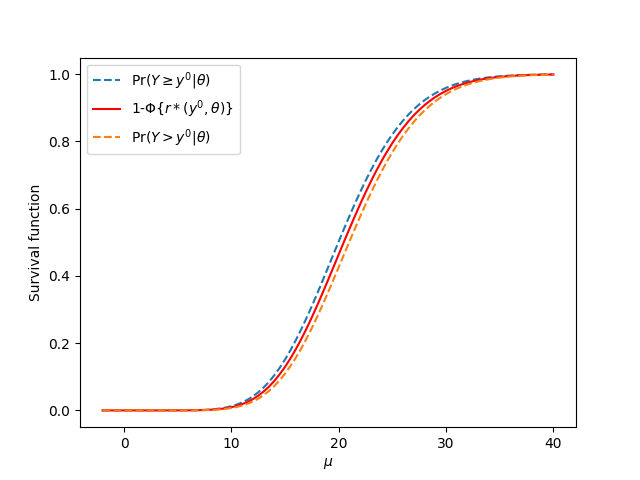
\includegraphics[width=0.7\textwidth]{Book_examples/book_sig.png}
	\caption{Survival function for Poisson distribution with observed sample $y^0=27$ for the upper limit, lower limit, and approximation $\Phi\{r^*(y^0,\mu)\}$}\label{fig:book_sf}
\end{figure} 
\newpage\noindent From these results its already apparent that the modification of the likelihood root is a great approximation, even to the first order. But for the interests of HEP it would be of interest to perform further test to check whether this is an approximation that can be used in the field.

\subsection{Further comparisons}
The first comparison one can ask, is to first of all, see how the approximations fare compared to the naive approach, where we assume that the likelihood-root by itself is asymptotic. An updated version of Figure \ref{fig:book_cdf} is showcased in Figure \ref{fig:book_cdf_fr}. Here we also omit the lower limit as it is not of great interest in the field of HEP.
\begin{figure}[!ht]
	\centering
        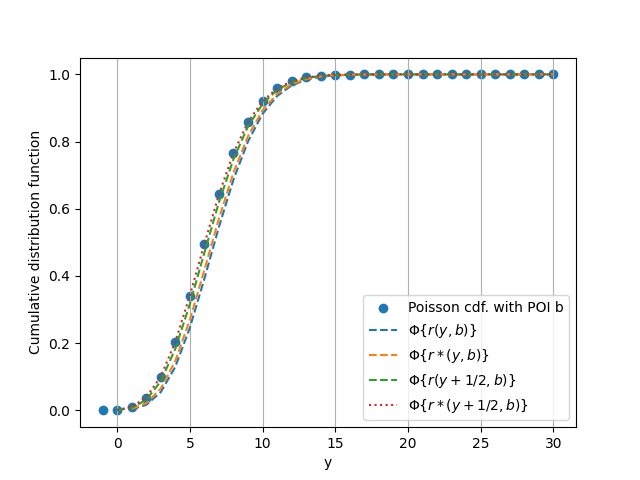
\includegraphics[width=0.7\textwidth]{Book_examples_further/book_cdf.png}
	\caption{Cumulative distribution function for Poisson distribution with parameter $b=6.7$ (scatter) with approximation $\Phi\{r^*(y,b)\}$ (dashed) and $\Phi\{r^*(y+1/2,b)\}$ (dotted)}\label{fig:book_cdf_fr}
\end{figure} 
And changing the y-axis on Figure \ref{fig:book_sf} to be the p-value, and showing all variants, we get Figure \ref{fig:book_sf_fr}.
\begin{figure}[!ht]
	\centering
        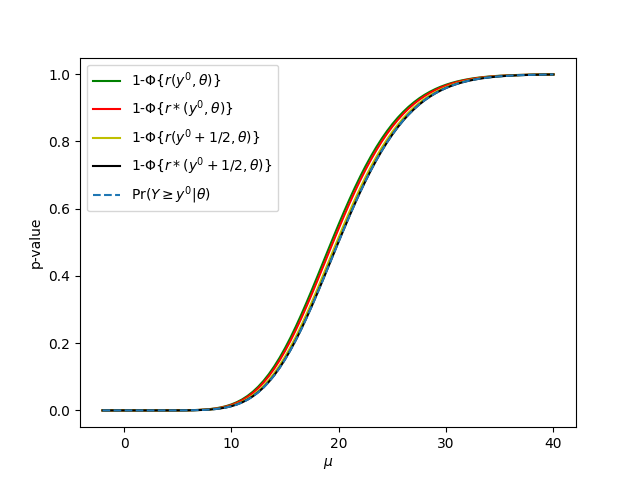
\includegraphics[width=0.7\textwidth]{Book_examples_further/book_sig.png}
	\caption{p-value for Poisson distribution with observed sample $y^0=27$ for the upper limit, lower limit, and approximation $\Phi\{r^*(y^0,\mu)\}$}\label{fig:book_sf_fr}
\end{figure} 
Which zoomed in on the upper tail, gives Figure \ref{fig:book_sf_fr_zoom}. \clearpage
\begin{figure}[!ht]
	\centering
        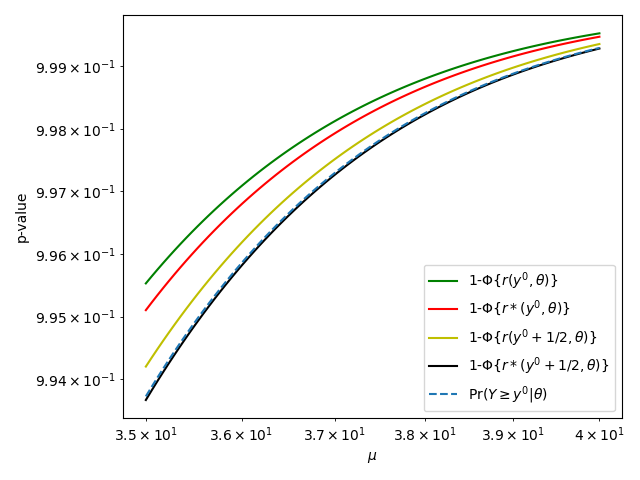
\includegraphics[width=0.7\textwidth]{Book_examples_further/book_sig_zoom.png}
	\caption{p-value for Poisson distribution with observed sample $y^0=27$ for the upper limit, lower limit, and approximation $\Phi\{r^*(y^0,\mu)\}$}\label{fig:book_sf_fr_zoom}
\end{figure} 
\noindent From this we can see that the most approximated (first order approximation with Mid-P) model seems overlap completely with the exact Poisson value. Something that is worth noting for the HEP field is that the other models give us a higher p-value compared to the exact ones, this is directly translated as having less significance, which means that if they were to be used they could possibly give us a Type-II error, meaning that we could say that the excess is not significant enough to exclude the null-hypothesis. \todo{Mention how toys come to play here? e.g. change r}

Because of the interest of this in  the field of HEP, we have conducted more tests to see how this approximation fares.



\subsubsection{$\chi^2_1$ comparison with Normal approximation with toys}
The first approximation is to check how the Central Limit Theorem applies to the test statistics at the minimum. Figure \ref{fig:nlls} shows how $t_\mu$ is distributed around the minima when setting $y=27$ and scanning over different $\mu$'s. 
\begin{figure}[!ht]
	\centering
        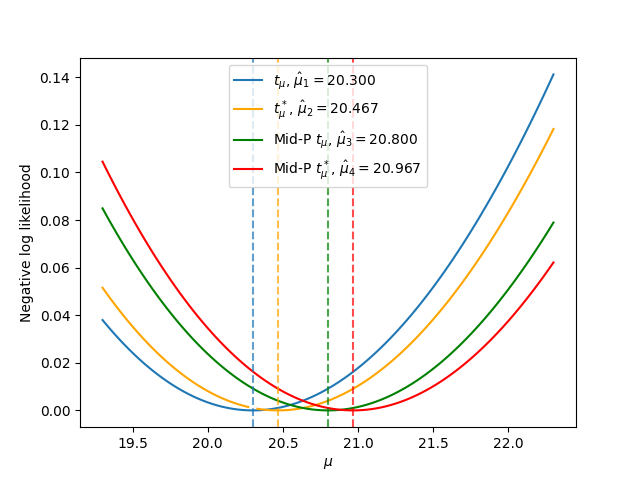
\includegraphics[width=0.5\textwidth]{Book_examples/nll_book.png}
	\caption{The test-statistics of all models we have for the Poisson example with $y=27$ and scanning over the signal strength $\mu$}\label{fig:nlls}
\end{figure} 
Around the minima, and as the number of samples increases, we expect that the distribution of the test statistics follows a standard normal with the mean at the minima\footnote{For this test we changed $\hat\mu=\hat\theta-b$, when in reality it should have been fixed at $\hat{\theta} = y^0=27$ for all models}, or mathematically
$$
f(t_\mu|\hat{\mu}) \sim\mathcal{N}(t_\mu|\hat{\mu}, 1)^2,
$$
which can be compared to a $\chi^2_1$ distribution. Figure \ref{fig:CLT} shows how toys generated from the above Normal distribution look, and how much they deviate from the $\chi^2_1$ distribution, we did this test for 1,000,000 and 100 toys.
\begin{figure}[!ht]
	\centering
	\begin{subfigure}[b]{0.49\textwidth}
        \centering
        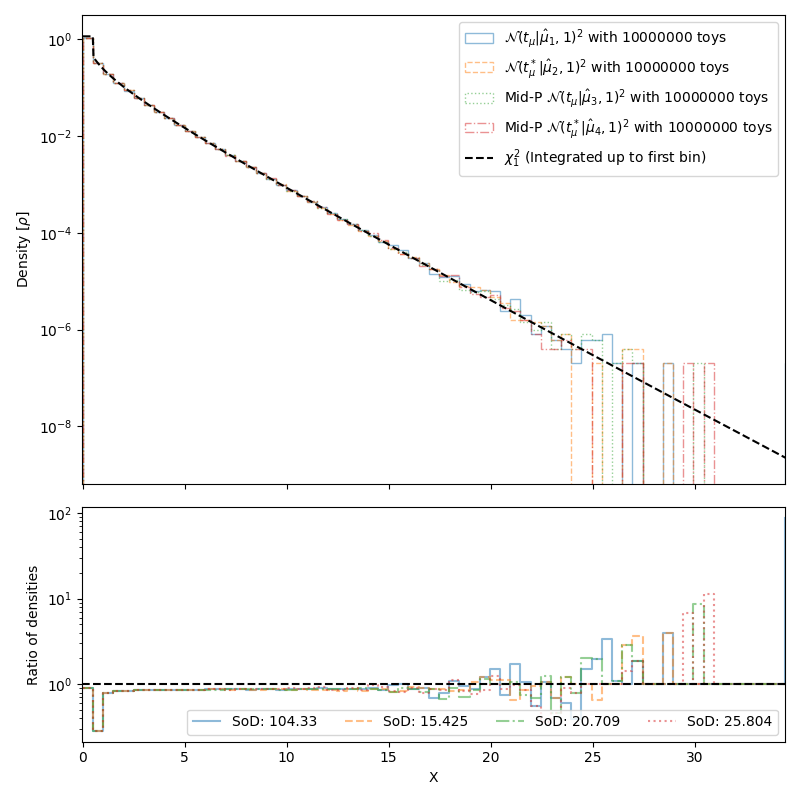
\includegraphics[width=1\textwidth]{CLT_diff_MLE/chi2_book_with_10000000_toys.png}
     \end{subfigure}
     \hfill
     \begin{subfigure}[b]{0.49\textwidth}
        \centering
        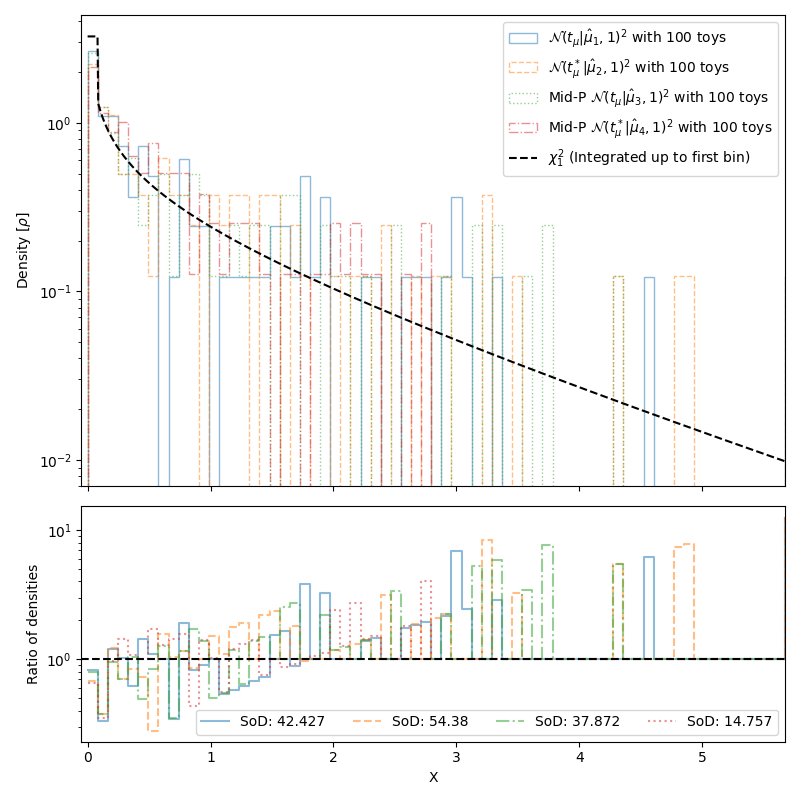
\includegraphics[width=1\textwidth]{CLT_diff_MLE/chi2_book_with_100_toys.png}
     \end{subfigure}
	\caption{PLACEHOLDER}\label{fig:CLT}
 \end{figure}

\subsubsection{$\chi^2_1$ comparison using the direct results}
The above test however, does not help avoid the use of toys. This another test is to generate events from the Poisson distribution at the $\theta=0$, and calculate the test-statistics at the null-hypothesis, $t_0$ for every event generated. The rundown on how this test was made, is that we calculated the test-statistics for every event in the distribution shown in Figure \ref{fig:example_dist}. The NLL for every $y$ is shown in Figure \ref{fig:example_nll0}. Then we can plot the test-statistic at the null-hypothesis for every event and every model, this is shown in Figure \ref{fig:example_nlls}.
\begin{figure}[!ht]
	\centering
        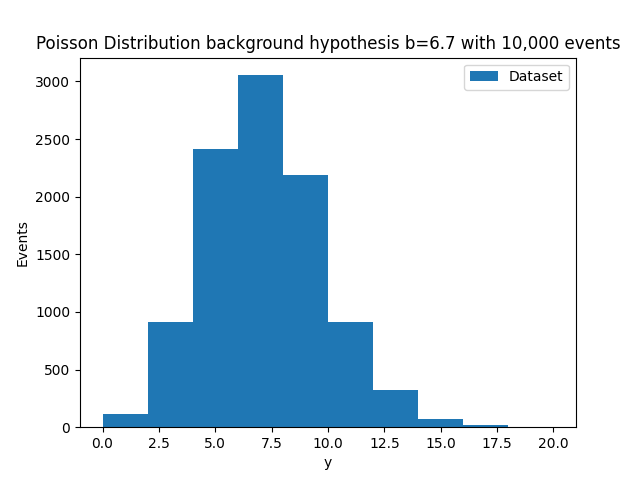
\includegraphics[width=0.6\textwidth]{Poisson_approximation_b6p7/distribution.png}\caption{Distribution used in test, $Y\sim\text{Poisson}(\theta=b=6.7)$}\label{fig:example_dist}
\end{figure} 
\begin{figure}[!ht]
	\centering
        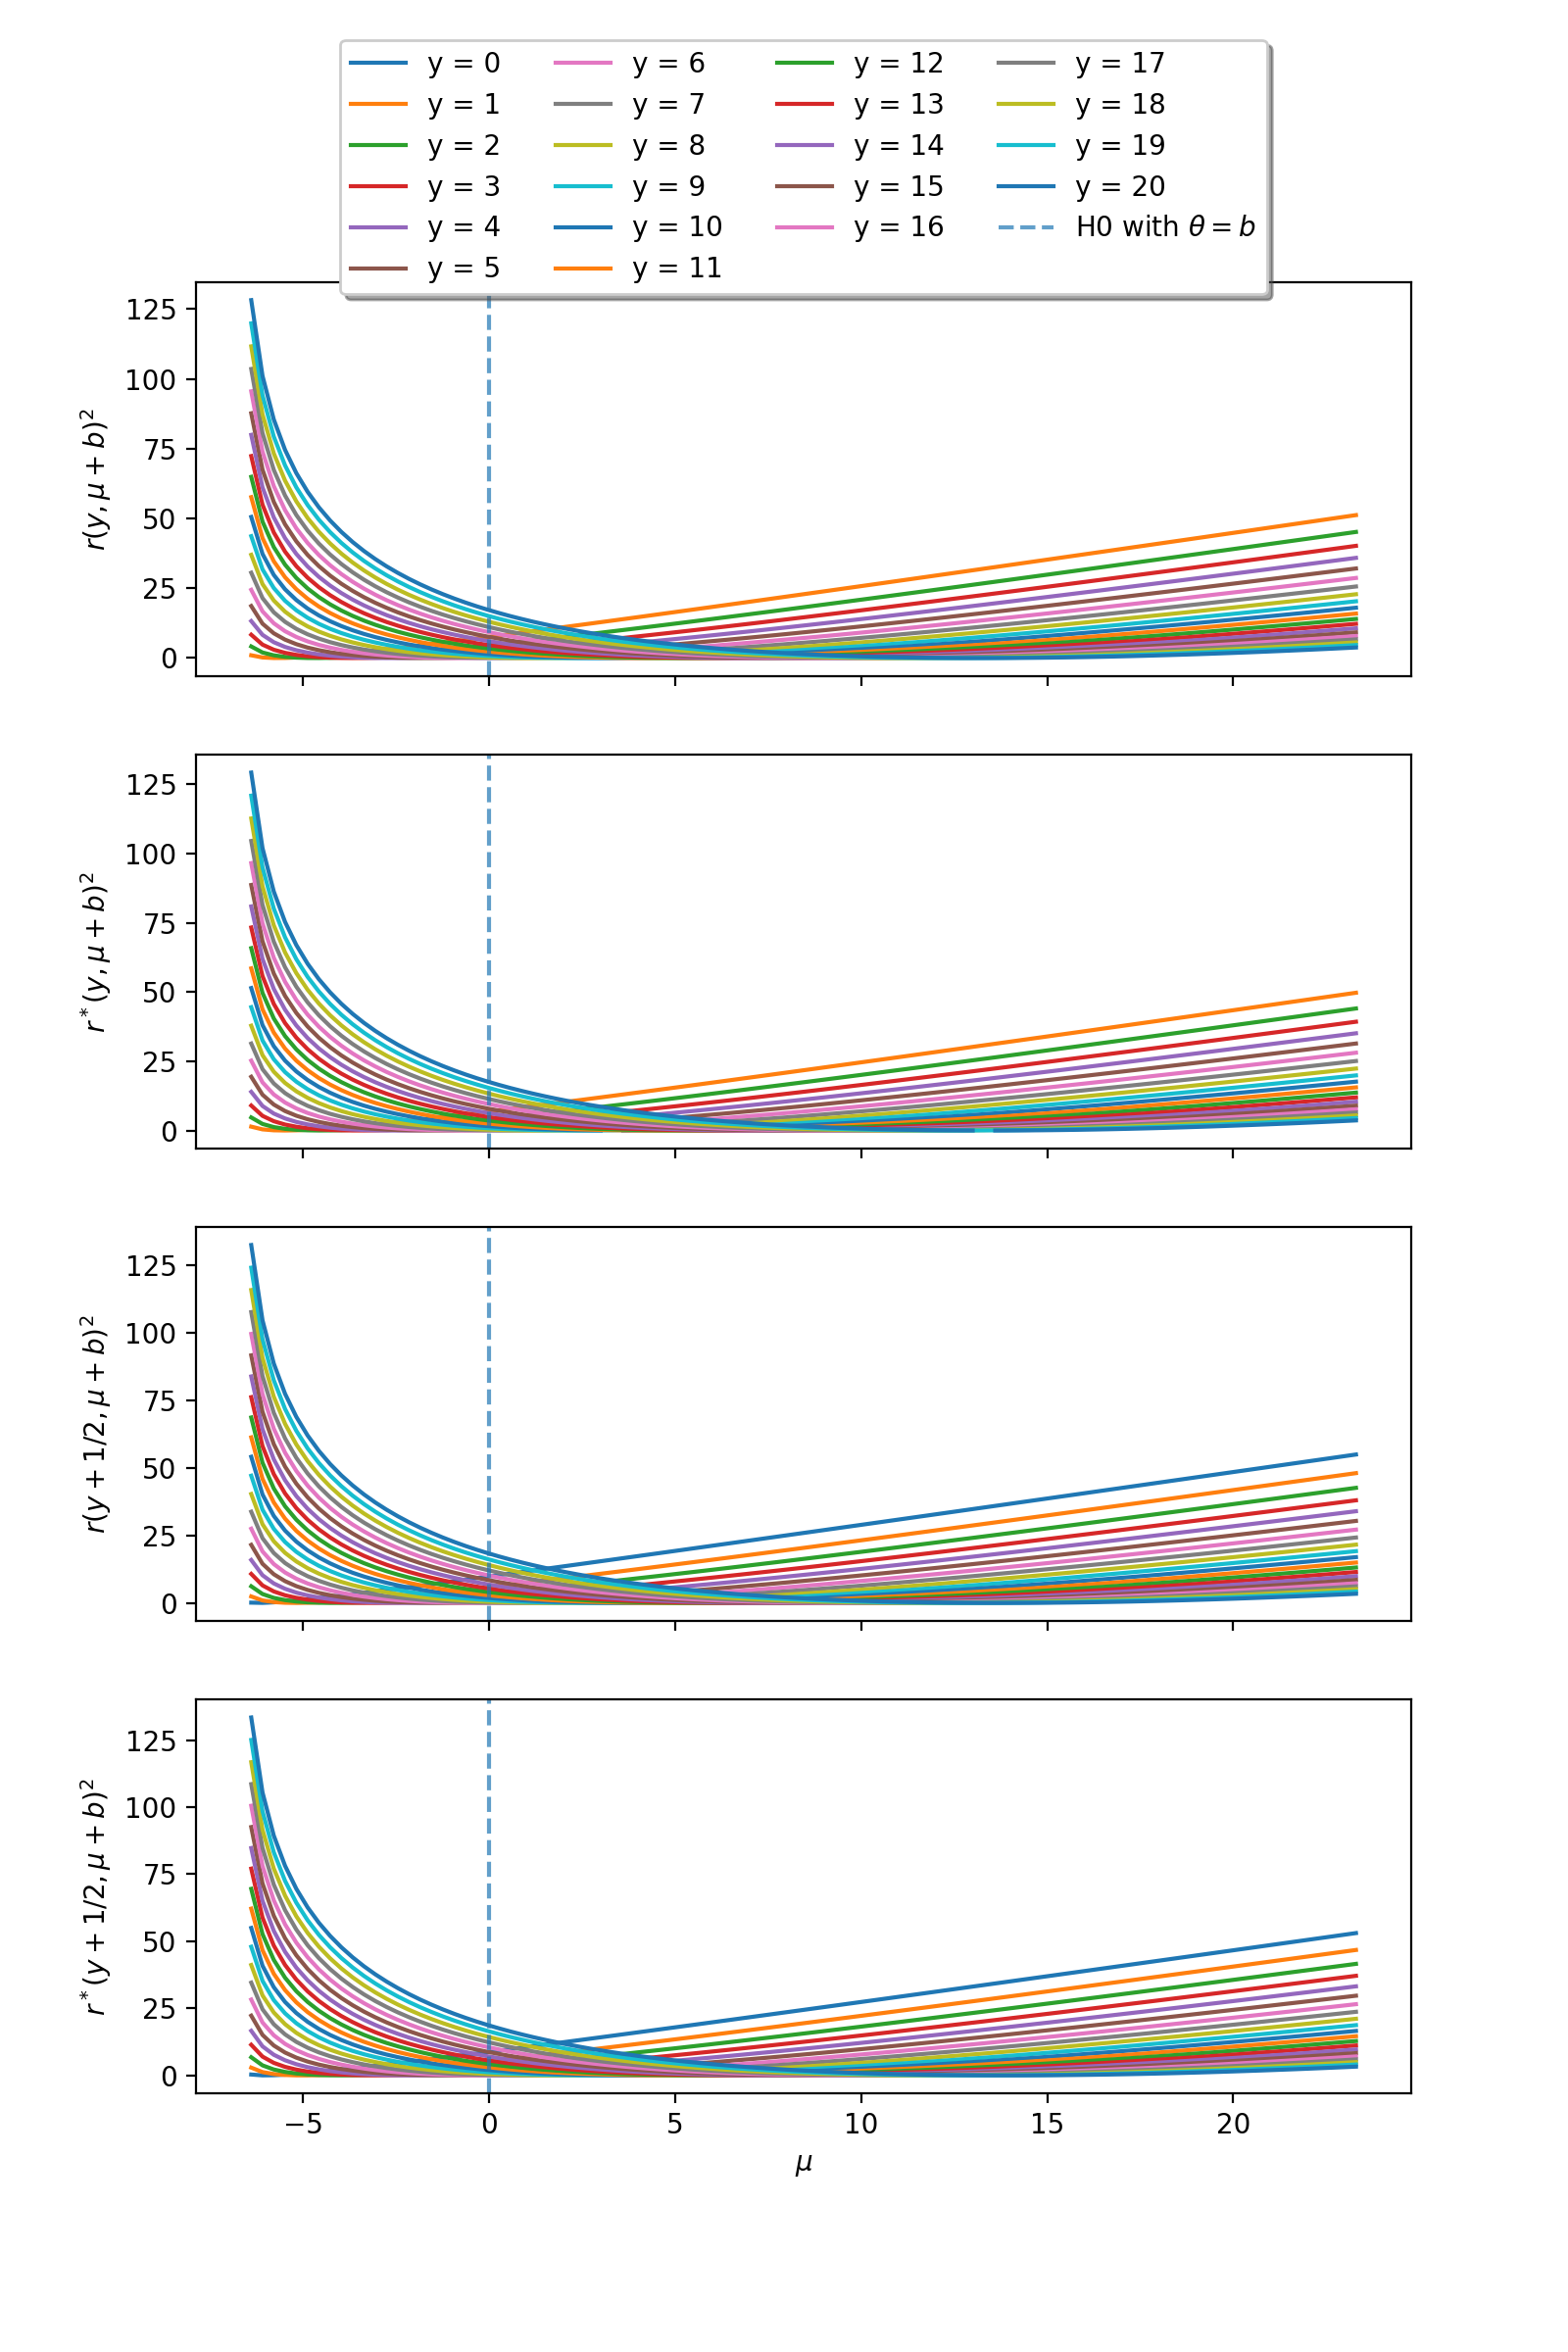
\includegraphics[width=0.7\textwidth]{Poisson_approximation_b6p7/nlls_event.png}\caption{Test statistics for every event in the example distribution with every model. The dashed blue line is the where the null-hypothesis is.}\label{fig:example_nlls}
\end{figure} 
\clearpage
\begin{figure}[!ht]
	\centering
        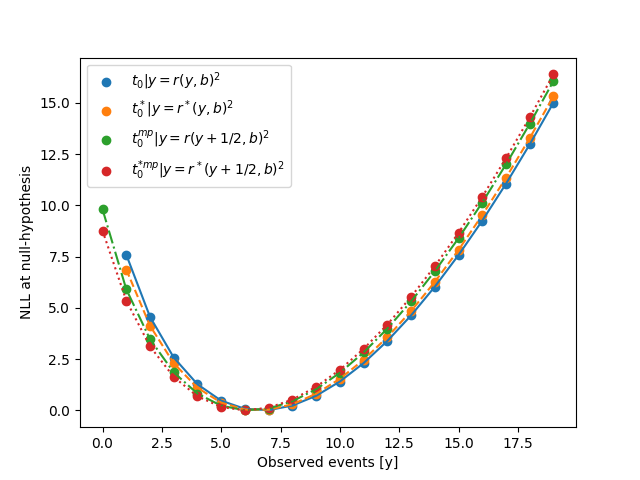
\includegraphics[width=0.6\textwidth]{OLD/image.png}\caption{Test statistics at the null-hypothesis for every event with every model}\label{fig:example_nll0}
\end{figure} 
From this, we can then plot the distribution of $f(t_0|y)$ for every model, and compare how this distribution looks for every generated event. This is shown in Figure \ref{fig:example_chisqr} for the example distribution. From this we see that the non Mid-P approximation is closer to a $\chi^2_1$ distribution when simulating 10,000 events. However, when repeating this experiment, but when only generating 10 events instead of 10,000 the most modified model performs better, shown in Figure \ref{fig:example_chisqr_10}.
\begin{figure}[!ht]
	\centering
        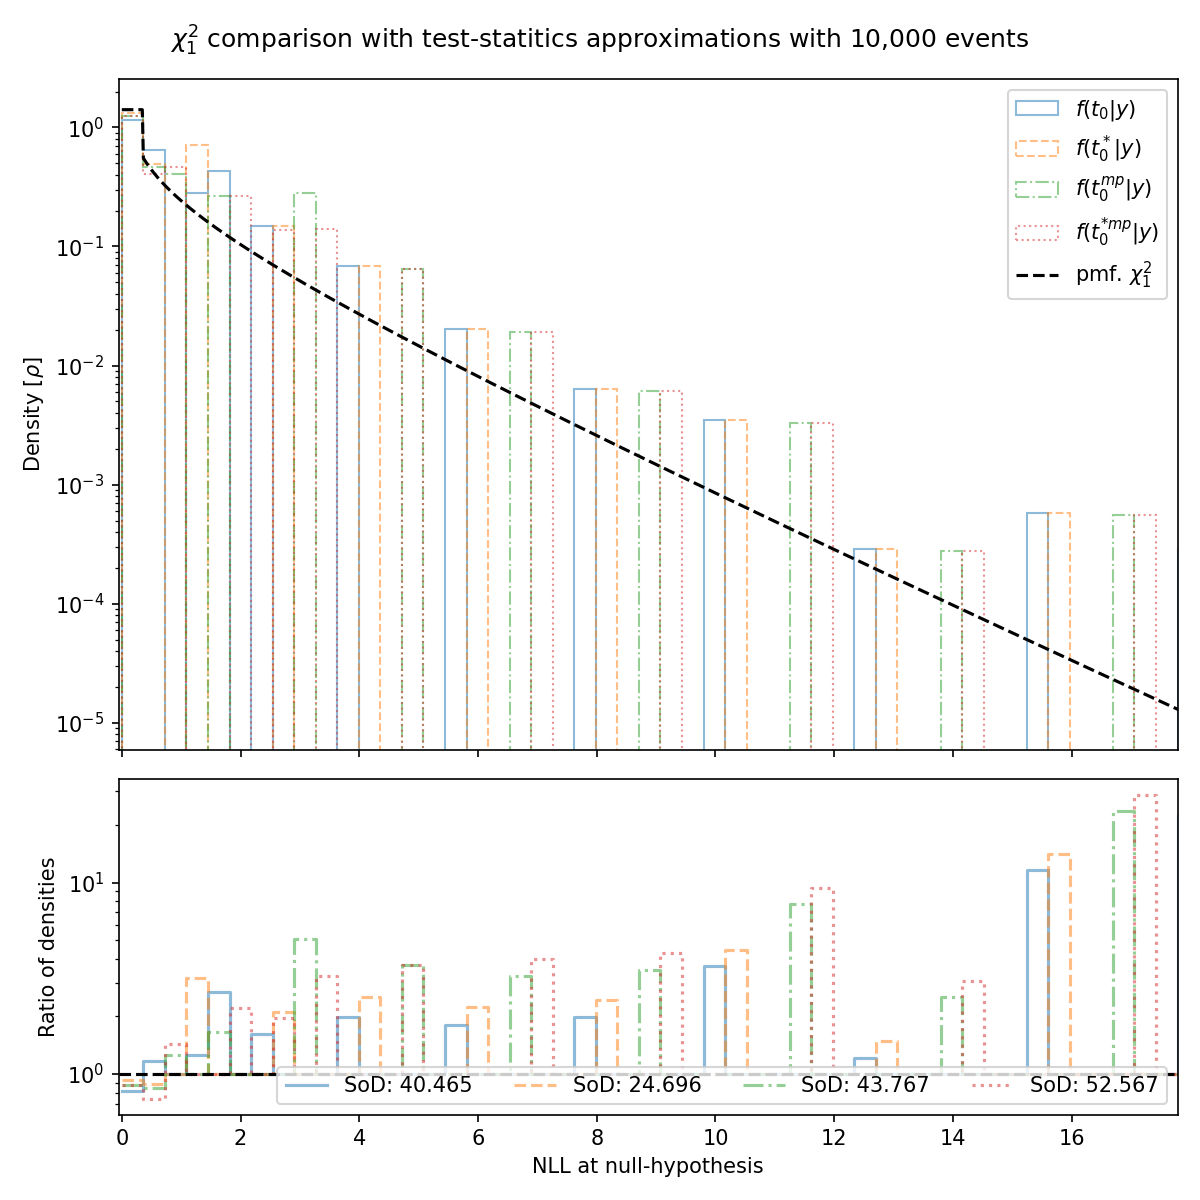
\includegraphics[width=0.7\textwidth]{Poisson_approximation_b2p997/NLL_densities.png}\caption{Upper plot: Distribution of test statistics at the null-hypothesis for every event with every model. Lower plot: deviation of models from $\chi^2_1$, and the Sum of Deviations (SoD) }\label{fig:example_chisqr}
\end{figure} 
\begin{figure}[!ht]
	\centering
        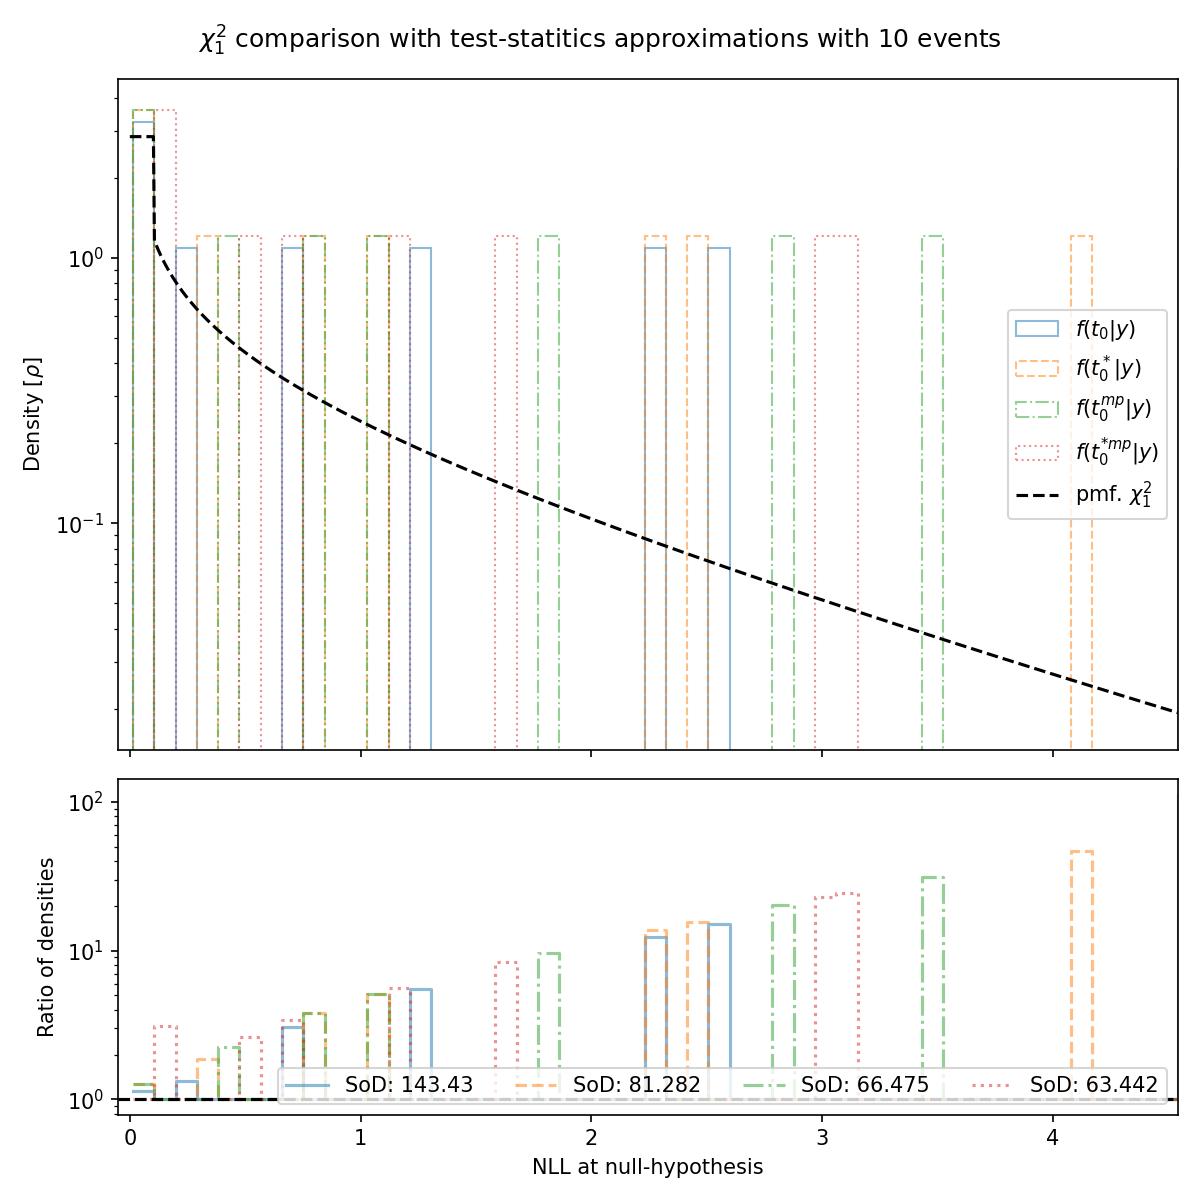
\includegraphics[width=0.7\textwidth]{OLD/NLL_densities.png}\caption{Upper plot: Distribution of test statistics at the null-hypothesis for every event with every model. Lower plot: deviation of models from $\chi^2_1$, and the Sum of Deviations (SoD) }\label{fig:example_chisqr_10}
\end{figure} 
\clearpage

\subsubsection{P-value comparison}
Another test one can conduct is to see how the p-value differs between models at the background hypothesis, using the same dataset from Figure \ref{fig:example_dist} we can recreate the p-value plot from Figure \ref{fig:book_sf_fr}, but instead of keeping the sample fixed, we keep the POI fixed at $\theta=b=6.7$. This is shown in Figure \ref{fig:example_pval}. Additionally, if we change the definition of the test statistics to better match the HEP convention of searching for excesses, then we can modify Figure \ref{fig:example_nll0} to only look at values for $\theta<\hat{\theta}$,\todo{cite cowan and cramner} this is shown in Figure \ref{fig:example_nll0_fr}.
\begin{figure}[!ht]
	\centering
	\begin{subfigure}[b]{0.49\textwidth}
        \centering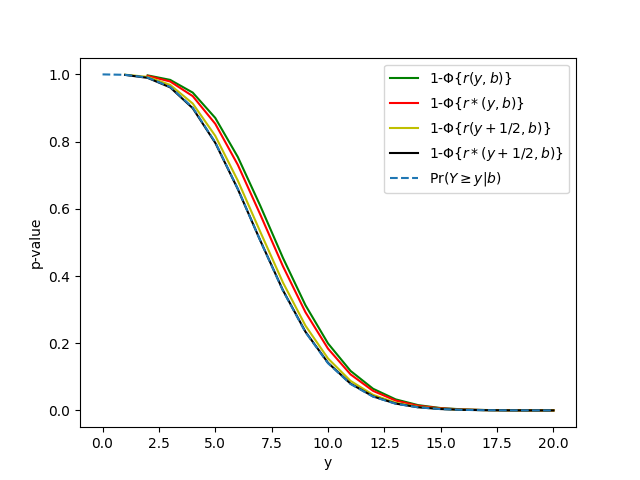
\includegraphics[width=1\textwidth]{Poisson_approximation_b6p7/p_values.png}\caption{P-value of each model, compared to the exact p-value of the Poisson. }\label{fig:example_pval}
     \end{subfigure}
     \hfill
     \begin{subfigure}[b]{0.49\textwidth}
        \centering
        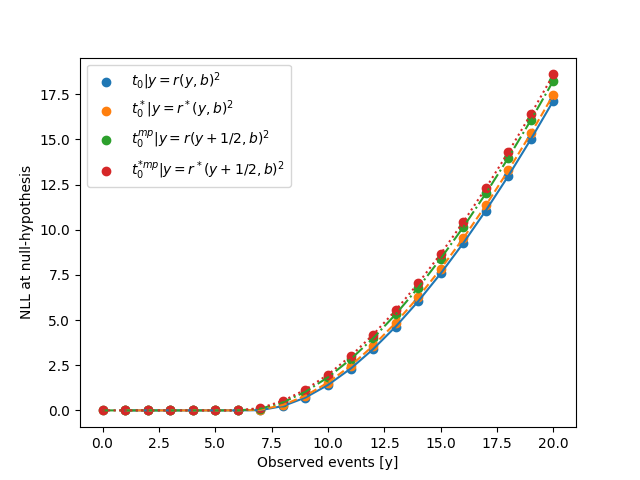
\includegraphics[width=1\textwidth]{Poisson_approximation_b6p7/NLL_null.png}\caption{Updated test-statistics at null-hypothesis plot that prioritizes searches. }\label{fig:example_nll0_fr}
     \end{subfigure}
	\caption{PLACEHOLDER}
 \end{figure}
 If we plot now the p-value for every model, at $t_0|y$ (naive model), then we can have a better look at how well the models are at finding estimating the true values. This is shown in Figure \ref{fig:example_p0}.
\begin{figure}[!ht]
	\centering
        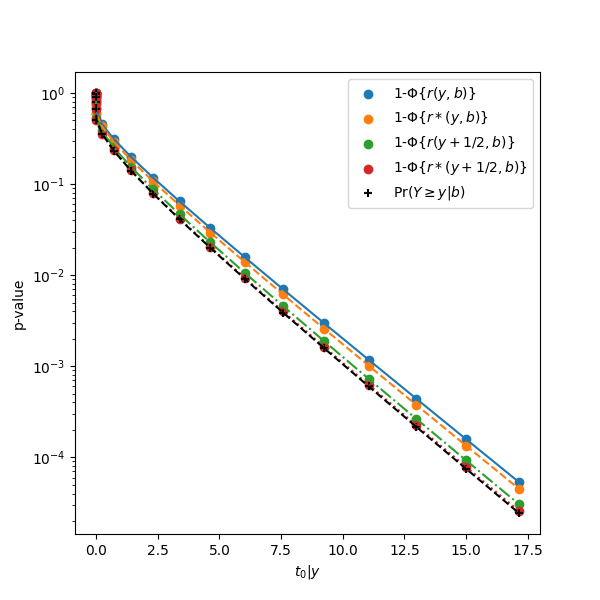
\includegraphics[width=0.7\textwidth]{Poisson_approximation_b6p7/p_values_vs_nom_2NLL.png}\caption{p-value vs -2NLL plot for every model}\label{fig:example_p0}
\end{figure} 
\clearpage\noindent From this we see that the most modified model performs almost exactly as the exact solution. But to further quantify this, we calculated it for other values of the POI. The results are shown in the Tables below
\begin{table}[!ht]
    \centering
    \caption{Table showcasing the experiment result for each unique value of y when setting the POI of a Poisson to b=6.7. The table shows (in this order) The p-value calculated using the approximated likelihood-root with Mid-P, the exact p-value of the Poisson distribution, the square root of the test statistics for the naive model in the background only hypothesis ($\sqrt{t_0|y}$), the effective $\sqrt{t_0|y}$ is the significance calculated from the p-value from the exact Poisson distribution using $Z = \Phi(1-p)$, $\sqrt{t_0^{*mp}|y}$ is the significance calculated from the most modified test statistics, and the effective $\sqrt{t_0^{*mp}|y}$ is calculated using the p-value of the most modified likelihood-root.}
    \begin{tabular}{lrrrrrr}
\toprule
 & Mid-P r* (p-value) & Poisson p-value & $\sqrt{t_0\vert y}$ & Effective $\sqrt{t_0\vert y}$ & $\sqrt{t_0^{*mp}\vert y}$ & Effective $\sqrt{t_0^{*mp}\vert y}$ \\
\midrule
0 & NaN & 1.000000 & NaN & -inf & 0.000000 & NaN \\
1 & 0.998465 & 0.998769 & 0.000000 & -3.027995 & 0.000000 & -2.960611 \\
2 & 0.989691 & 0.990522 & 0.000000 & -2.346394 & 0.000000 & -2.314912 \\
3 & 0.961412 & 0.962894 & 0.000000 & -1.785306 & 0.000000 & -1.767310 \\
4 & 0.899365 & 0.901192 & 0.000000 & -1.288374 & 0.000000 & -1.277944 \\
5 & 0.796292 & 0.797841 & 0.000000 & -0.833934 & 0.000000 & -0.828448 \\
6 & 0.658627 & 0.659351 & 0.000000 & -0.410691 & 0.000000 & -0.408718 \\
7 & 0.504967 & 0.504703 & 0.115051 & -0.011789 & 0.364626 & -0.012450 \\
8 & 0.357695 & 0.356683 & 0.487180 & 0.367339 & 0.725572 & 0.364626 \\
9 & 0.234050 & 0.232716 & 0.843864 & 0.729930 & 1.072684 & 0.725572 \\
10 & 0.141706 & 0.140430 & 1.187245 & 1.078389 & 1.407737 & 1.072684 \\
11 & 0.079605 & 0.078598 & 1.518990 & 1.414563 & 1.732139 & 1.407737 \\
12 & 0.041624 & 0.040937 & 1.840429 & 1.739914 & 2.047034 & 1.732139 \\
13 & 0.020327 & 0.019910 & 2.152647 & 2.055620 & 2.353367 & 2.047034 \\
14 & 0.009302 & 0.009072 & 2.456541 & 2.362652 & 2.651928 & 2.353367 \\
15 & 0.004002 & 0.003886 & 2.752868 & 2.661822 & 2.943387 & 2.651928 \\
16 & 0.001623 & 0.001569 & 3.042269 & 2.953817 & 3.228322 & 2.943387 \\
17 & 0.000623 & 0.000599 & 3.325297 & 3.239223 & 3.507230 & 3.228322 \\
18 & 0.000226 & 0.000217 & 3.602431 & 3.518550 & 3.780546 & 3.507230 \\
19 & 0.000078 & 0.000075 & 3.874093 & 3.792240 & 4.048655 & 3.780546 \\
20 & 0.000026 & 0.000024 & 4.140651 & 4.060683 & 4.311896 & 4.048655 \\
\bottomrule
\end{tabular}

\end{table}

\begin{table}[!ht]
    \centering
    \caption{Table showcasing the experiment result for each unique value of y when setting the POI of a Poisson to b=2.997. The table shows (in this order) The p-value calculated using the approximated likelihood-root with Mid-P, the exact p-value of the Poisson distribution, the square root of the test statistics for the naive model in the background only hypothesis ($\sqrt{t_0|y}$) the effective $\sqrt{t_0|y}$ is the significance calculated from the p-value from the exact Poisson distribution using $Z = \Phi(1-p)$, $\sqrt{t_0^{*mp}|y}$ is the significance calculated from the most modified test statistics, and the effective $\sqrt{t_0^{*mp}|y}$ is calculated using the p-value of the most modified likelihood-root.}
    \begin{tabular}{lrrrrrr}
\toprule
 & Mid-P r* (p-value) & Poisson p-value & $\sqrt{t_0\vert y}$ & Effective $\sqrt{t_0\vert y}$ & $\sqrt{t_0^{*mp}\vert y}$ & Effective $\sqrt{t_0^{*mp}\vert y}$ \\
\midrule
0 & NaN & 1.000000 & NaN & -inf & 0.000000 & NaN \\
1 & 0.944804 & 0.950063 & 0.000000 & -1.645468 & 0.000000 & -1.596429 \\
2 & 0.796820 & 0.800403 & 0.000000 & -0.843062 & 0.000000 & -0.830315 \\
3 & 0.576068 & 0.576137 & 0.001733 & -0.192022 & 0.373163 & -0.191845 \\
4 & 0.354514 & 0.352096 & 0.550873 & 0.379668 & 0.888679 & 0.373163 \\
5 & 0.187088 & 0.184233 & 1.054638 & 0.899351 & 1.367647 & 0.888679 \\
6 & 0.085711 & 0.083616 & 1.524392 & 1.381154 & 1.818041 & 1.367647 \\
7 & 0.034529 & 0.033358 & 1.967277 & 1.833589 & 2.245213 & 1.818041 \\
8 & 0.012377 & 0.011840 & 2.388153 & 2.262288 & 2.652975 & 2.245213 \\
9 & 0.003989 & 0.003779 & 2.790525 & 2.671225 & 3.044165 & 2.652975 \\
10 & 0.001167 & 0.001094 & 3.177022 & 3.063339 & 3.420965 & 3.044165 \\
11 & 0.000312 & 0.000290 & 3.549681 & 3.440878 & 3.785103 & 3.420965 \\
12 & 0.000077 & 0.000071 & 3.910125 & 3.805614 & 4.137973 & 3.785103 \\
13 & 0.000018 & 0.000016 & 4.259669 & 4.158973 & 4.480722 & 4.137973 \\
\bottomrule
\end{tabular}

\end{table}

\begin{table}[!ht]
    \centering
     \caption{Table showcasing the experiment result for each unique value of y when setting the POI of a Poisson to b=0.78. The table shows (in this order) The p-value calculated using the approximated likelihood-root with Mid-P, the exact p-value of the Poisson distribution, the square root of the test statistics for the naive model in the background only hypothesis ($\sqrt{t_0|y}$) the effective $\sqrt{t_0|y}$ is the significance calculated from the p-value from the exact Poisson distribution using $Z = \Phi(1-p)$, $\sqrt{t_0^{*mp}|y}$ is the significance calculated from the most modified test statistics, and the effective $\sqrt{t_0^{*mp}|y}$ is calculated using the p-value of the most modified likelihood-root.}
    \begin{tabular}{lrrrrrr}
\toprule
 & Mid-P r* (p-value) & Poisson p-value & $\sqrt{t_0\vert y}$ & Effective $\sqrt{t_0\vert y}$ & $\sqrt{t_0^{*mp}\vert y}$ & Effective $\sqrt{t_0^{*mp}\vert y}$ \\
\midrule
0 & NaN & 1.000000 & NaN & -inf & 0.000000 & NaN \\
1 & 0.545018 & 0.541594 & 0.238585 & -0.104450 & 0.865249 & -0.113083 \\
2 & 0.193451 & 0.184037 & 1.151709 & 0.900086 & 1.658140 & 0.865249 \\
3 & 0.048645 & 0.044590 & 1.908518 & 1.699737 & 2.349571 & 1.658140 \\
4 & 0.009398 & 0.008334 & 2.576441 & 2.393953 & 2.974312 & 2.349571 \\
5 & 0.001468 & 0.001264 & 3.184178 & 3.019976 & 3.550594 & 2.974312 \\
\bottomrule
\end{tabular}

\end{table}

\section{Concluision so far}
Need NPs!!

 
\newpage
\printbibliography
\end{document}
